\section{Boundary Value Problem Frameworks}

%%%%%%%%%%%%%%%%%%%%%%%%%%%%%%%%%%%%%%%%%%%%%%%%%%%%%%%%%%%%%%%%%%%%%
\royslide{Boundary Value Problem Framework Goals}{
Goals:
\royitemizebegin
\item Improving test coverage and reliability
\item Hiding of implementation details from user code
\item Rapid prototyping of differential equation approximations
\item Improved error estimation
\royitemizeend

Methods:
\royitemizebegin
\item Object-oriented System and Solver classes
\item Numerical Jacobian verification
\royitemizeend
}

%%%%%%%%%%%%%%%%%%%%%%%%%%%%%%%%%%%%%%%%%%%%%%%%%%%%%%%%%%%%%%%%%%%%%
\royslide{FEM System Classes}{

\begin{minipage}[h]{.45\textwidth}
\begin{center}
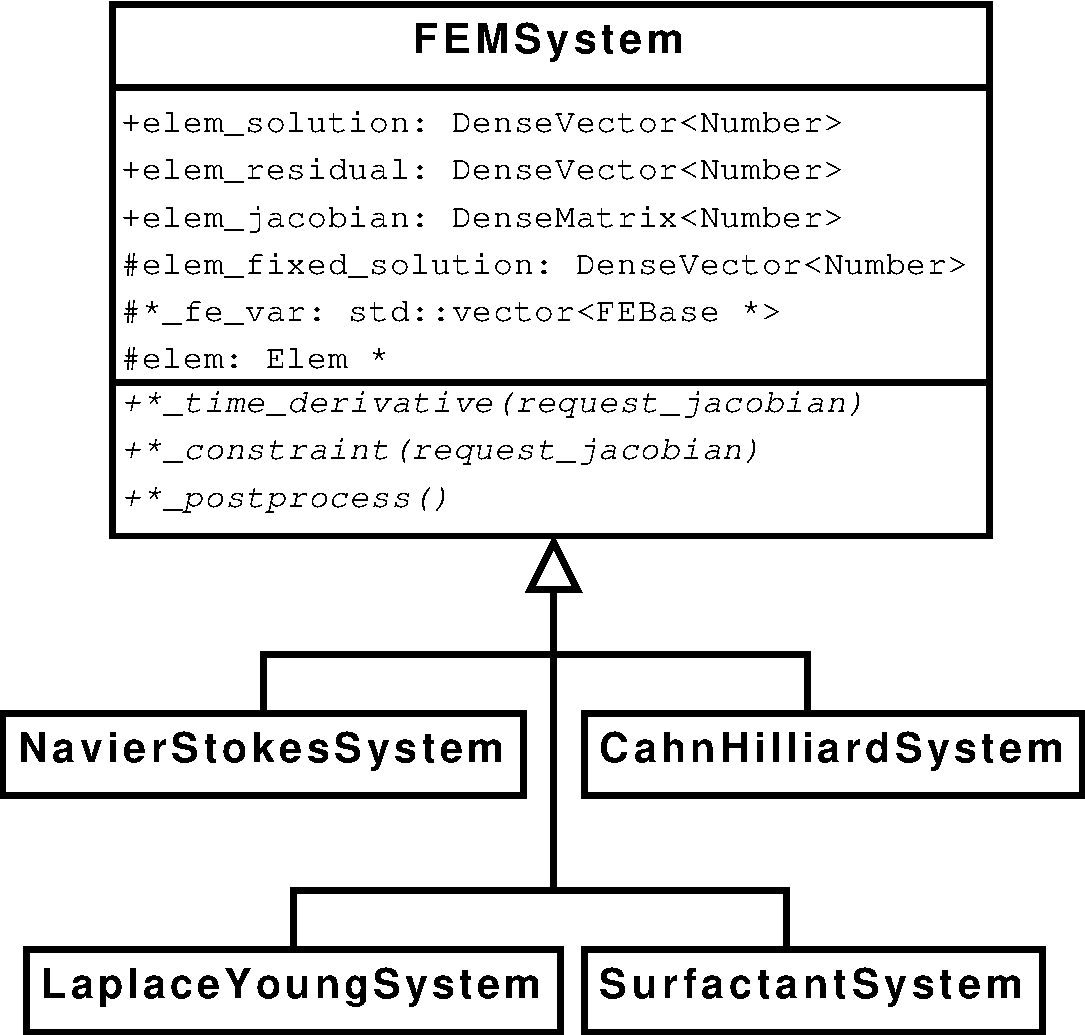
\includegraphics[width=.9\textwidth]{figs/FEMSystem}
\end{center}
\end{minipage}
\begin{minipage}[h]{.45\textwidth}
\royitemizebegin
\item Generalized IBVP representation
\item FEMSystem does all initialization, global assembly
\item User code only needs weighted time derivative residuals
$(\dt{u}, v_i) = F_i(u)$ and/or constraints $G_i(u, v_i) = 0$
\royitemizeend
\end{minipage}

}

%%%%%%%%%%%%%%%%%%%%%%%%%%%%%%%%%%%%%%%%%%%%%%%%%%%%%%%%%%%%%%%%%%%%%
\royslide{ODE Solver Classes}{

\begin{minipage}[h]{.45\textwidth}
\begin{center}
\includegraphics[width=.9\textwidth]{figs/TimeSolver}
\end{center}
\end{minipage}
\begin{minipage}[h]{.45\textwidth}
\royitemizebegin
\item Calls user code on each element
\item Assembles element-by-element time derivatives, constraints, and weighted
old solutions
\royitemizeend
\end{minipage}

}

%%%%%%%%%%%%%%%%%%%%%%%%%%%%%%%%%%%%%%%%%%%%%%%%%%%%%%%%%%%%%%%%%%%%%
\royslide{Nonlinear Solver Classes}{

\begin{minipage}[h]{.45\textwidth}
\begin{center}
\includegraphics[width=.9\textwidth]{figs/NonlinearSolver}
\end{center}
\end{minipage}
\begin{minipage}[h]{.45\textwidth}
\royitemizebegin
\item Acquires residuals, jacobians from FEMSystem assembly
\item Handles inner loops, inner solvers and tolerances, convergence tests, etc
\royitemizeend
\end{minipage}

}

%%%%%%%%%%%%%%%%%%%%%%%%%%%%%%%%%%%%%%%%%%%%%%%%%%%%%%%%%%%%%%%%%%%%%
\royslide{Element-based BVP Framework}{

Pros:
\royitemizebegin
\item Enables non-global physics-based error estimators
\item Removes dependencies, complications from application level
\item Gives user access to more tested code
\item Enables element-by-element Jacobian verification
\royitemizeend

Cons:
\royitemizebegin
\item Adds additional per-element virtual function calls
\item Complicates time-dependent stabilization methods
\item Complicates operator splitting methods
\royitemizeend

}
